% Options for packages loaded elsewhere
\PassOptionsToPackage{unicode}{hyperref}
\PassOptionsToPackage{hyphens}{url}
%
\documentclass[
  8pt,
  ignorenonframetext,
]{beamer}
\usepackage{pgfpages}
\setbeamertemplate{caption}[numbered]
\setbeamertemplate{caption label separator}{: }
\setbeamercolor{caption name}{fg=normal text.fg}
\beamertemplatenavigationsymbolsempty
% Prevent slide breaks in the middle of a paragraph
\widowpenalties 1 10000
\raggedbottom
\setbeamertemplate{part page}{
  \centering
  \begin{beamercolorbox}[sep=16pt,center]{part title}
    \usebeamerfont{part title}\insertpart\par
  \end{beamercolorbox}
}
\setbeamertemplate{section page}{
  \centering
  \begin{beamercolorbox}[sep=12pt,center]{part title}
    \usebeamerfont{section title}\insertsection\par
  \end{beamercolorbox}
}
\setbeamertemplate{subsection page}{
  \centering
  \begin{beamercolorbox}[sep=8pt,center]{part title}
    \usebeamerfont{subsection title}\insertsubsection\par
  \end{beamercolorbox}
}
\AtBeginPart{
  \frame{\partpage}
}
\AtBeginSection{
  \ifbibliography
  \else
    \frame{\sectionpage}
  \fi
}
\AtBeginSubsection{
  \frame{\subsectionpage}
}
\usepackage{amsmath,amssymb}
\usepackage{lmodern}
\usepackage{iftex}
\ifPDFTeX
  \usepackage[T1]{fontenc}
  \usepackage[utf8]{inputenc}
  \usepackage{textcomp} % provide euro and other symbols
\else % if luatex or xetex
  \usepackage{unicode-math}
  \defaultfontfeatures{Scale=MatchLowercase}
  \defaultfontfeatures[\rmfamily]{Ligatures=TeX,Scale=1}
\fi
% Use upquote if available, for straight quotes in verbatim environments
\IfFileExists{upquote.sty}{\usepackage{upquote}}{}
\IfFileExists{microtype.sty}{% use microtype if available
  \usepackage[]{microtype}
  \UseMicrotypeSet[protrusion]{basicmath} % disable protrusion for tt fonts
}{}
\makeatletter
\@ifundefined{KOMAClassName}{% if non-KOMA class
  \IfFileExists{parskip.sty}{%
    \usepackage{parskip}
  }{% else
    \setlength{\parindent}{0pt}
    \setlength{\parskip}{6pt plus 2pt minus 1pt}}
}{% if KOMA class
  \KOMAoptions{parskip=half}}
\makeatother
\usepackage{xcolor}
\newif\ifbibliography
\setlength{\emergencystretch}{3em} % prevent overfull lines
\providecommand{\tightlist}{%
  \setlength{\itemsep}{0pt}\setlength{\parskip}{0pt}}
\setcounter{secnumdepth}{-\maxdimen} % remove section numbering
% type setting
% ------------------------------------------------------------------------------
\usepackage[german]{babel}     

% fonts
% ------------------------------------------------------------------------------
\usefonttheme{professionalfonts}

% slide title and horizontal line
% ------------------------------------------------------------------------------
\setbeamertemplate{frametitle}{%
    \vskip-30pt \color{black}\large%
    \begin{minipage}[b][23pt]{120mm}%
    \flushleft\insertframetitle%
    \end{minipage}%
}

\setbeamertemplate{headline}										
{
\vskip10pt\hfill\hspace{3.5mm} 										 
\vskip15pt\color{black}\rule{\textwidth}{0.4pt} 					 
}

% slide number
% ---------------------------------------------------------------
\setbeamertemplate{navigation symbols}{}
\setbeamertemplate{footline}
{
\vskip5pt
\vskip2pt
\makebox[123mm]{\hspace{7.5mm}
\hfill Wahrscheinlichkeitstheorie und Frequentistische Inferenz $\vert$ 
\copyright $ $ 2023 Dirk Ostwald CC BY-SA 4.0 $\vert$ 
Folie \insertframenumber}
\vskip4pt
}

% block color scheme
% ------------------------------------------------------------------------------
% colors
\definecolor{white}{RGB}{255,255,255}
\definecolor{grey}{RGB}{235,235,235}
\definecolor{lightgrey}{RGB}{245,245,245}
\definecolor{LightBlue}{RGB}{220,220,255}
\definecolor{darkblue}{RGB}{51, 51, 153}

% definitions and theorems
\setbeamercolor{block title}{fg = black, bg = grey}
\setbeamercolor{block body}{fg = black, bg = lightgrey}

% general line spacing 
% ------------------------------------------------------------------------------
\linespread{1.3}

% local line spacing
% ------------------------------------------------------------------------------
\usepackage{setspace}

% colors
% -----------------------------------------------------------------------------
\usepackage{color}

% justified text
% ------------------------------------------------------------------------------
\usepackage{ragged2e}
\usepackage{etoolbox}
\apptocmd{\frame}{}{\justifying}{}
\usepackage{ragged2e}
\renewcommand{\raggedright}{\justifying}

% bullet point lists
% -----------------------------------------------------------------------------
\setbeamertemplate{itemize item}[circle]
\setbeamertemplate{itemize subitem}[circle]
\setbeamertemplate{itemize subsubitem}[circle]
\setbeamercolor{itemize item}{fg = black}
\setbeamercolor{itemize subitem}{fg = black}
\setbeamercolor{itemize subsubitem}{fg = black}
\setbeamercolor{enumerate item}{fg = black}
\setbeamercolor{enumerate subitem}{fg = black}
\setbeamercolor{enumerate subsubitem}{fg = black}
\setbeamerfont{itemize/enumerate body}{}
\setbeamerfont{itemize/enumerate subbody}{size = \normalsize}
\setbeamerfont{itemize/enumerate subsubbody}{size = \normalsize}

% color links
% ------------------------------------------------------------------------------
\usepackage{hyperref}
\definecolor{urls}{RGB}{204,0,0}
\hypersetup{colorlinks, citecolor = darkblue, urlcolor = urls}


% additional math commands
% ------------------------------------------------------------------------------
\usepackage{bm}                                         % bold math symbols
\newcommand{\niton}{\not\owns}

% text highlighting
% ------------------------------------------------------------------------------
\usepackage{soul}
\makeatletter
\let\HL\hl
\renewcommand\hl{%
  \let\set@color\beamerorig@set@color
  \let\reset@color\beamerorig@reset@color
  \HL}
\makeatother

% equation highlighting
% -----------------------------------------------------------------------------
\newcommand{\highlight}[2][yellow]{\mathchoice%
  {\colorbox{#1}{$\displaystyle#2$}}%
  {\colorbox{#1}{$\textstyle#2$}}%
  {\colorbox{#1}{$\scriptstyle#2$}}%
  {\colorbox{#1}{$\scriptscriptstyle#2$}}}%

% additional mathematical operators
% ------------------------------------------------------------------------------
\DeclareMathOperator*{\argmax}{arg\,max}
\DeclareMathOperator*{\argmin}{arg\,min}

\ifLuaTeX
  \usepackage{selnolig}  % disable illegal ligatures
\fi
\IfFileExists{bookmark.sty}{\usepackage{bookmark}}{\usepackage{hyperref}}
\IfFileExists{xurl.sty}{\usepackage{xurl}}{} % add URL line breaks if available
\urlstyle{same} % disable monospaced font for URLs
\hypersetup{
  hidelinks,
  pdfcreator={LaTeX via pandoc}}

\author{}
\date{\vspace{-2.5em}}

\begin{document}

\begin{frame}[plain]{}
\protect\hypertarget{section}{}
\center

\begin{center}
\includegraphics[width=0.2\linewidth]{3_Abbildungen/wtfi_3_otto} \end{center}

\vspace{2mm}

\Large

Wahrscheinlichkeitstheorie und Frequentistische Inferenz \vspace{6mm}

\large

BSc Psychologie WiSe 2022/23

\vspace{6mm}
\large

Prof.~Dr.~Dirk Ostwald
\end{frame}

\begin{frame}[plain]{}
\protect\hypertarget{section-1}{}
\vfill
\center
\huge

\textcolor{black}{(3) Elementare Wahrscheinlichkeiten} \vfill
\end{frame}

\begin{frame}{}
\protect\hypertarget{section-2}{}
\begin{center}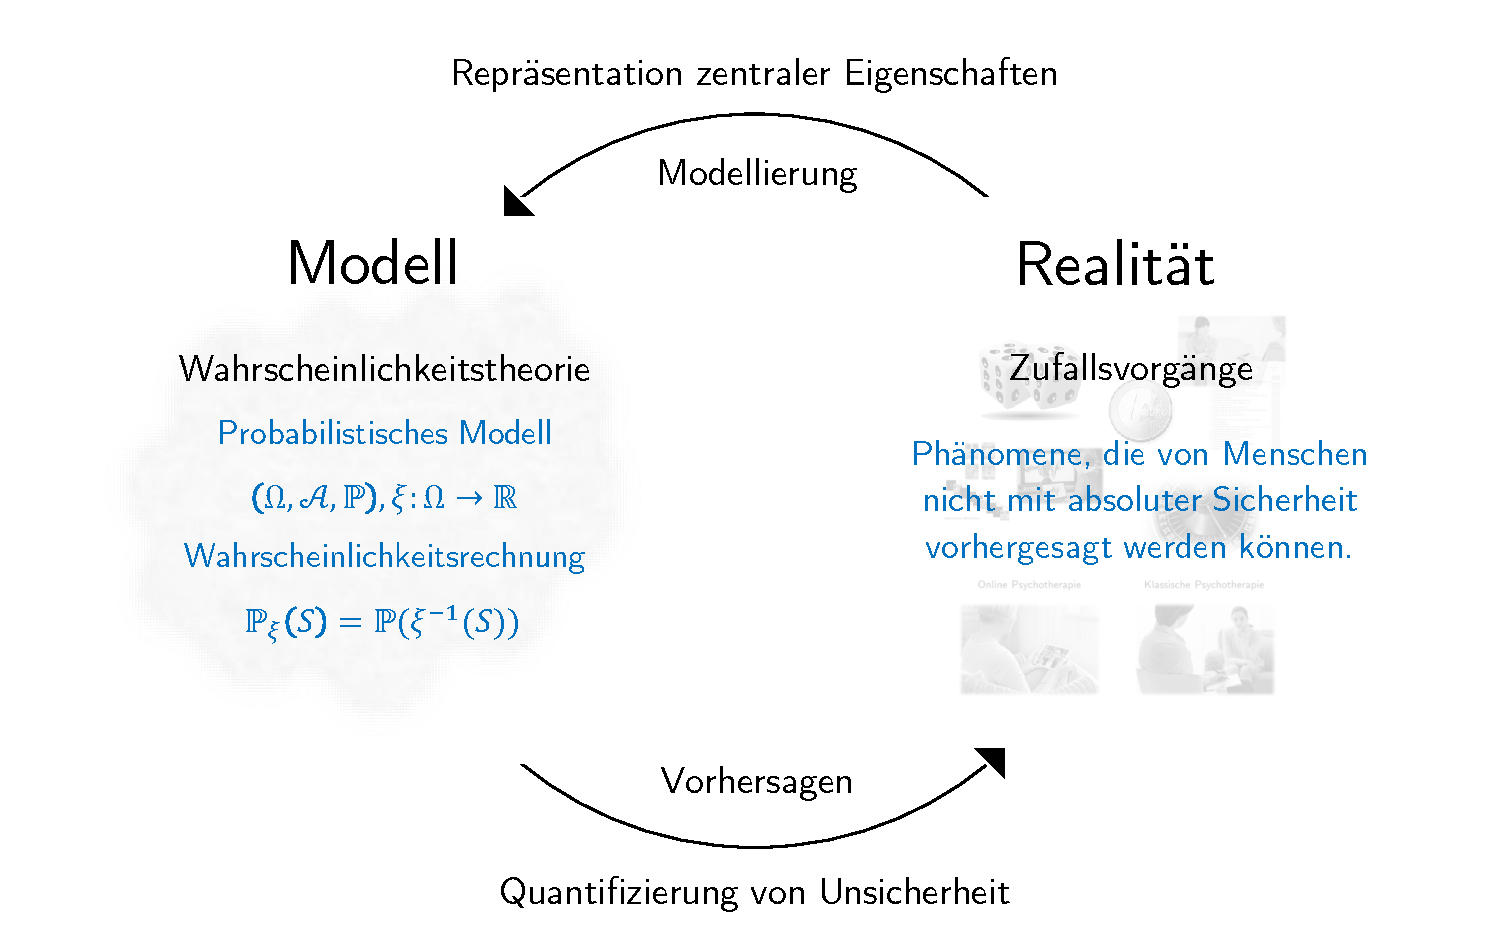
\includegraphics[width=0.9\linewidth]{3_Abbildungen/wtfi_3_wahrscheinlichkeitstheorie_modell} \end{center}
\end{frame}

\begin{frame}{}
\protect\hypertarget{section-3}{}
\begin{center}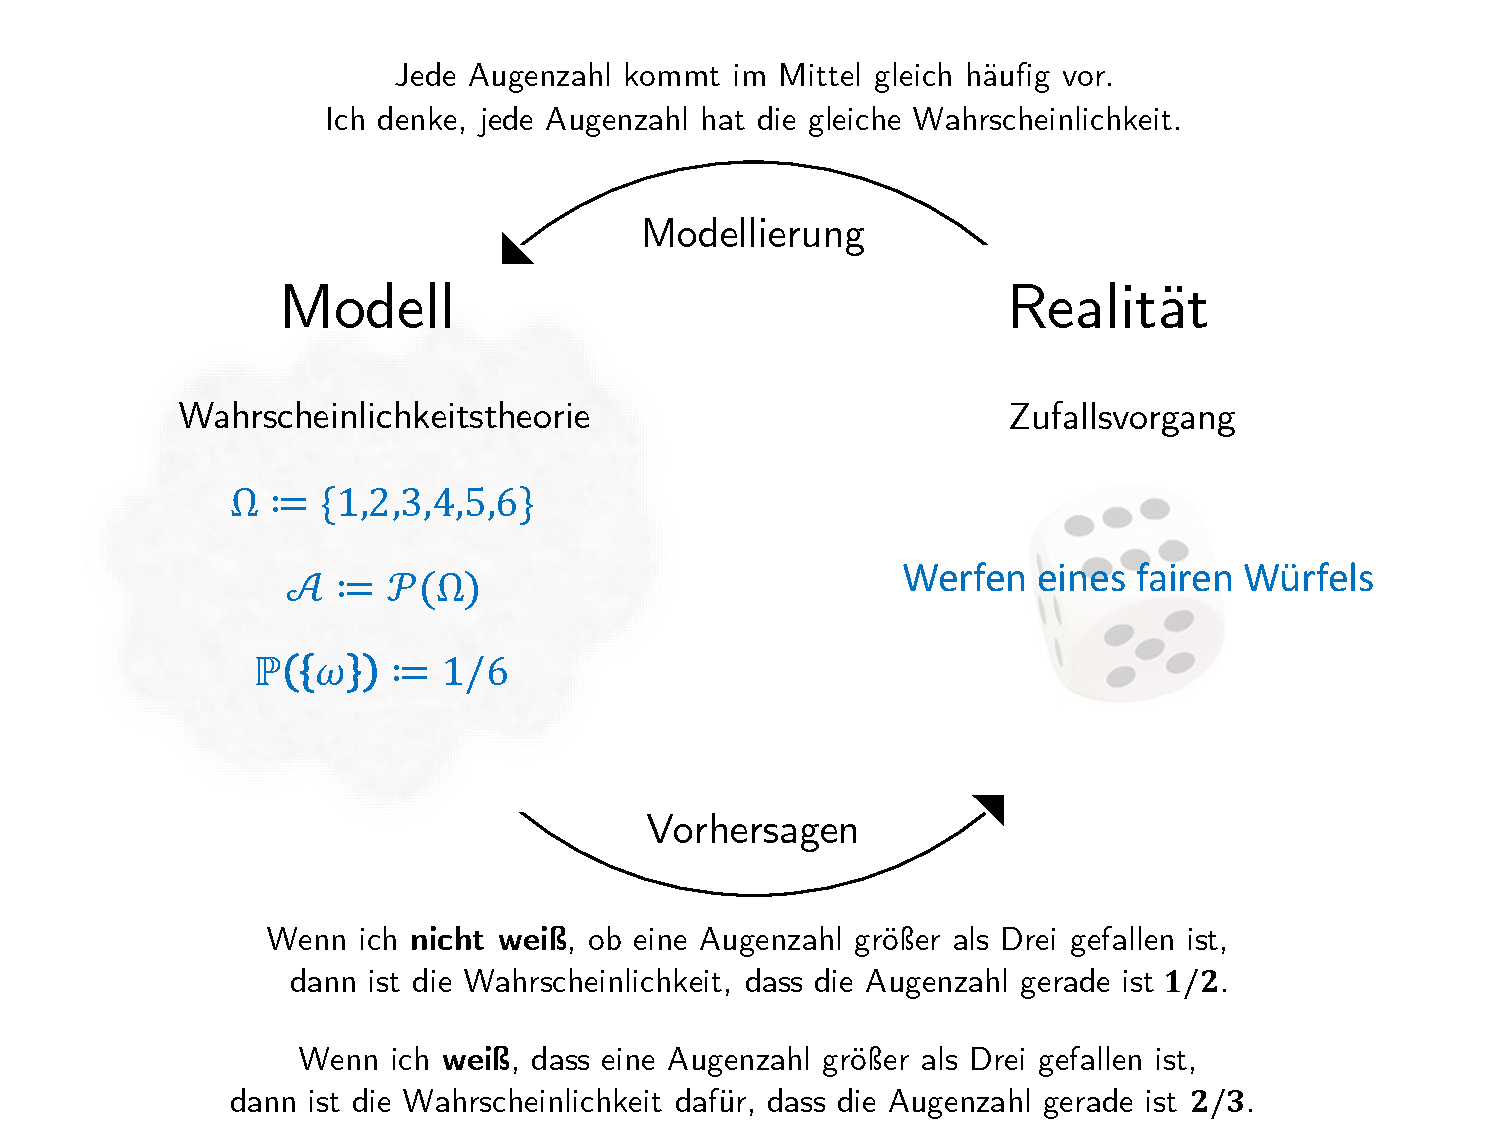
\includegraphics[width=0.9\linewidth]{3_Abbildungen/wtfi_3_wahrscheinlichkeitstheorie_modell_beispiel} \end{center}
\end{frame}

\begin{frame}{}
\protect\hypertarget{section-4}{}
\setstretch{2}
\vfill
\large

Interpretation

Gemeinsame Wahrscheinlichkeiten

Weitere Eigenschaften

Unabhängige Ereignisse

Bedingte Wahrscheinlichkeiten

Selbstkontrollfragen \vfill
\end{frame}

\begin{frame}{}
\protect\hypertarget{section-5}{}
\setstretch{2}
\vfill
\large

\textbf{Interpretation}

Gemeinsame Wahrscheinlichkeiten

Weitere Eigenschaften

Unabhängige Ereignisse

Bedingte Wahrscheinlichkeiten

Selbstkontrollfragen \vfill
\end{frame}

\begin{frame}{Interpretation}
\protect\hypertarget{interpretation}{}
Wiederholung der Definition

\small

Es seien \(\Omega\) eine Ereignismenge und \(\mathcal{A}\) eine
\(\sigma\)-Algebra auf \(\Omega\). Eine Abbildung \begin{equation}
\mathbb{P} : \mathcal{A} \to [0,1], A \mapsto \mathbb{P}(A)
\end{equation} mit den Eigenschaften

\begin{itemize}
\item $\mathbb{P}(A) \ge 0$ für alle $A \in \mathcal{A}$ (Nicht-Negativität),
\item $\mathbb{P}(\Omega) = 1$ (Normiertheit),
\item $\mathbb{P}\left(\cup_{i=1}^\infty A_i\right) = \sum_{i=1}^\infty \mathbb{P}(A_i)$
für paarweise disjunkte $A_i \in \mathcal{A}$ ($\sigma$-Additivität)
\end{itemize}

heißt ein \textit{Wahrscheinlichkeitsmaß} oder einfach
\textit{Wahrscheinlichkeit}. Der Funktionswert \(\mathbb{P}(A)\) heißt
\textit{Wahrscheinlichkeit des Ereignisses
$A \in \mathcal{A}$}.
\end{frame}

\begin{frame}{Interpretation}
\protect\hypertarget{interpretation-1}{}
\small

In der W-Theorie sind Wahrscheinlichkeiten anhand ihrer mathematischen
Eigenschaften definiert.

Die Interpretation des mathematischen Wahrscheinlichkeitsbegriffs
\(\mathbb{P}(A)\) ist nicht eindeutig.

Es gibt mindestens zwei unterschiedliche Interpretationen:

Nach der \textbf{Frequentistischen Interpretation} ist \(\mathbb{P}(A)\)
die idealisierte relative Häufigkeit, mit der das Ereignis \(A\) unter
den gleichen äußeren Bedingungen einzutreten pflegt. Zum Beispiel ist
die frequentistische Interpretation von \(\mathbb{P}(\{6\})\) im Modell
des Werfen eines Würfels ``Wenn man einen Würfel unendlich oft werfen
würde und die relative Häufigkeit des Elementareignisses \(\{6\}\)
bestimmen würde, dann wäre diese relative Häufigkeit gleich
\(\mathbb{P}(\{6\})\).''

Nach der \textbf{Bayesianischen Interpretation} ist \(\mathbb{P}(A)\)
der Grad der Sicherheit, den eine Beobachter:in aufgrund ihrer
subjektiven Einschätzung der Lage dem Eintreten des Ereignisses \(A\)
zumisst. Zum Beispiel ist die Bayesianische Interpretation von
\(\mathbb{P}(\{6\})\) im Modell des Werfen eines Würfels ``Basierend auf
meinen Erfahrung mit dem Werfen eines Würfels bin ich mir zu
\(\mathbb{P}(\{6\})\cdot 100\) Prozent sicher, dass der Würfel beim
nächsten Wurf eine 6 zeigt.''
\end{frame}

\begin{frame}{Interpretation}
\protect\hypertarget{interpretation-2}{}
\small

In Modellen von tatsächlich wiederholbaren Zufallsvorgängen wie dem
Werfen eines Würfels ist der Unterschied zwischen Frequentistischer und
Bayesianischer Interpretation eher subtil. Es gibt aber viele
Zufallsvorgänge, die mit Wahrscheinlichkeiten beschrieben werden, bei
denen aufgrund ihrer Einmaligkeit eine frequentistische Interpretation
jedoch nicht sinnvoll ist. Zum Beispiel machen Aussagen der Form ``Die
Wahrscheinlichkeit, dass sich die Temperatur der Erde bis zum Jahr 2100
nur um 2° Celsius erhöht, wenn der CO\(_2\) Ausstoß sofort auf Null
gesetzt würde, ist 0.5'' nur unter der Bayesianischen Interpretation
Sinn.

In Hinblick auf die Definitionen und Rechenregeln für
Wahrscheinlichkeiten unterscheiden sich beide Interpretationen
allerdings nicht. Sowohl die frequentistische als auch die Bayesianisch
geprägte probabilistische Datenanalyse haben mit der
Wahrscheinlichkeitstheorie ein identisches mathematisches Bezugssystem.

Wir werden also erst an späterer Stelle wieder auf unterschiedliche
Herangehensweisen in der probabilistischen Datenanalyse, die sich aus
den unterschiedlichen Interpretation des Wahrscheinlichkeitsbegriffes
ergeben, zurückkommen.

Generell kann man vielleicht sagen, dass die Bayesianische
Interpretation mathematischer Wahrscheinlichkeiten logisch schlüssiger
ist, in vielen wichtigen Anwendungsfeldern wie der Psychologie oder
Biomedizin, frequentistisch geprägte Datenanalysen aber weiterhin
vorherrschen.
\end{frame}

\begin{frame}{}
\protect\hypertarget{section-6}{}
\setstretch{2}
\vfill
\large

Interpretation

\textbf{Gemeinsame Wahrscheinlichkeiten}

Weitere Eigenschaften

Unabhängige Ereignisse

Bedingte Wahrscheinlichkeiten

Selbstkontrollfragen \vfill
\end{frame}

\begin{frame}{Gemeinsame Wahrscheinlichkeiten}
\protect\hypertarget{gemeinsame-wahrscheinlichkeiten}{}
\small
\begin{definition}[Gemeinsame Wahrscheinlichkeit]
\justifying
$(\Omega, \mathcal{A}, \mathbb{P})$ sei ein Wahrscheinlichkeitsraum und es seien
$A,B \in \mathcal{A}$. Dann heißt
\begin{equation}
\mathbb{P}(A \cap B)
\end{equation}
die \textit{gemeinsame Wahrscheinlichkeit von $A$ und $B$}.
\end{definition}

\setstretch{1.5}

Bemerkungen

\begin{itemize}
\tightlist
\item
  Zur Abgrenzung nennt man \(\mathbb{P}(A)\) auch manchmal auch
  \emph{totale Wahrscheinlichkeit von \(A\)}.
\item
  Intuitiv entspricht \(\mathbb{P}(A \cap B)\) der Wahrscheinlichkeit,
  dass \(A\) und \(B\) gleichzeitig eintreten.
\item
  In der Mechanik des W-Raummodells ist \(\mathbb{P}(A \cap B)\) die
  Wahrscheinlichkeit, dass in einem Durchgang des Zufallsvorgang ein
  \(\omega\) mit sowohl \(\omega \in A\) und \(\omega \in B\) realisiert
  wird.
\end{itemize}
\end{frame}

\begin{frame}{Gemeinsame Wahrscheinlichkeiten}
\protect\hypertarget{gemeinsame-wahrscheinlichkeiten-1}{}
Beispiel

\small

\begin{itemize}
\item
  Wir betrachten das Wahrscheinlichkeitsraummodells des Werfens eines
  fairen Würfels.
\item
  Wir betrachten die Ereignisse
\end{itemize}

\begin{center}
\begin{tabular}{ll}
$A := \{2,4,6\}$ & Es fällt eine gerade Augenzahl              \\
$B := \{4,5,6\}$ & Es fällt eine Augenzahl größer als Drei     \\
\end{tabular}
\end{center}

\begin{itemize}
\item
  Dann gilt \(A \cap B = \{4,6\}\).
\item
  Die Interpretation von \(A \cap B = \{4,6\}\) ist \center ``Es fällt
  eine gerade Augenzahl und diese Augenzahl ist größer als Drei.''
\end{itemize}

\justifying

\begin{itemize}
\tightlist
\item
  Mit \(\mathbb{P}(\{4\}) = \mathbb{P}(\{6\}) = 1/6\) und der
  \(\sigma\)-Additivität von \(\mathbb{P}\) ergibt sich \begin{align}
  \begin{split}
  \mathbb{P}(A \cap B)
  & = \mathbb{P}( \{2,4,6\} \cap \{4,5,6\})       \\
  & = \mathbb{P}( \{4,6\})                        \\
  & = \mathbb{P}(\{4\}) + \mathbb{P}(\{6\})       \\
  & = 1/6 + 1/6                                    \\
  & = 1/3.
  \end{split}
  \end{align}
\end{itemize}
\end{frame}

\begin{frame}{Gemeinsame Wahrscheinlichkeiten}
\protect\hypertarget{gemeinsame-wahrscheinlichkeiten-2}{}
Interpretation von \(\mathbb{P}(A \cup B)\) \small

\begin{itemize}
\begin{small}
\item $\mathbb{P}(A \cap B)$ und $\mathbb{P}(A \cup B)$ sollten nicht verwechselt werden.
\item $\cup$ entspricht dem \textit{inklusiven oder}, also \textit{und/oder}.
\item $\Delta$ entspricht dem \textit{exklusiven oder}, also \textit{entweder..., oder ..., aber nicht beides}.
\item $A \cup B$ entspricht also dem Ereignis, dass $A$ und/oder $B$ eintritt.
\item $\omega \in A \cup B$ ist also schon erfüllt, wenn ``nur'' $\omega \in A$ oder ``nur'' $\omega \in B$ gilt.
\item Für obiges Beispiel gilt
\begin{equation}
A \cup B = \{2,4,6\} \cup \{4,5,6\} = \{2,4,5,6\}
\end{equation}
mit der Interpretation
\end{small}
\end{itemize}

\center

``Es fällt eine gerade Augenzahl oder es fällt eine Augenzahl größer als
Drei

oder es fällt eine gerade Augenzahl und diese Augenzahl ist größer als
Drei''.

\justifying

\(\quad\,\,\,\) und der Wahrscheinlichkeit \begin{equation}
\mathbb{P}(\{2,4,5,6\}) = 4/6 = 2/3.
\end{equation}
\end{frame}

\begin{frame}{}
\protect\hypertarget{section-7}{}
\setstretch{2}
\vfill
\large

Interpretation

Gemeinsame Wahrscheinlichkeiten

\textbf{Weitere Eigenschaften}

Unabhängige Ereignisse

Bedingte Wahrscheinlichkeiten

Selbstkontrollfragen \vfill
\end{frame}

\begin{frame}{Weitere Eigenschaften}
\protect\hypertarget{weitere-eigenschaften}{}
\begin{theorem}[Weitere Eigenschaften von Wahrscheinlichkeiten]
\normalfont
\justifying
$(\Omega, \mathcal{A}, \mathbb{P})$ sei ein Wahrscheinlichkeitsraum und es seien
$A,B \in \mathcal{A}$ Ereignisse. Dann gelten
\begin{enumerate}
\itemsep2mm
\item $\mathbb{P}(A^c) = 1 - \mathbb{P}(A)$.
\item $A \subset B \Rightarrow \mathbb{P}(A) \le \mathbb{P}(B)$.
\item $\mathbb{P}(A \cap B^c) = \mathbb{P}(A) - \mathbb{P}(A \cap B)$
\item $\mathbb{P}(A \cup B) = \mathbb{P}(A) + \mathbb{P}(B) - \mathbb{P}(A \cap B)$.
\item $A \cap B = \emptyset \Rightarrow \mathbb{P}(A \cup B) = \mathbb{P}(A) + \mathbb{P}(B)$.
\end{enumerate}
\end{theorem}

\small

Bemerkungen

\begin{itemize}
\tightlist
\item
  Die Eigenschaften sind in der Analyse probabilistischer Modelle oft
  nützlich.
\end{itemize}
\end{frame}

\begin{frame}{Weitere Eigenschaften}
\protect\hypertarget{weitere-eigenschaften-1}{}
\footnotesize

\underline{Beweis}

Die zweite, dritte, und vierte Aussage dieses Theorems basieren auf
elementaren mengentheoretischen Aussagen und der \(\sigma\)-Addivität
von \(\mathbb{P}\). Wir wollen diese elementaren mengentheoretischen
Aussagen hier nicht beweisen, sondern verweisen jeweils auf die
Intuition, die durch die Venn-Diagramme in untenstehender Abbildung
vermittelt wird.

\vspace{2mm}

\begin{center}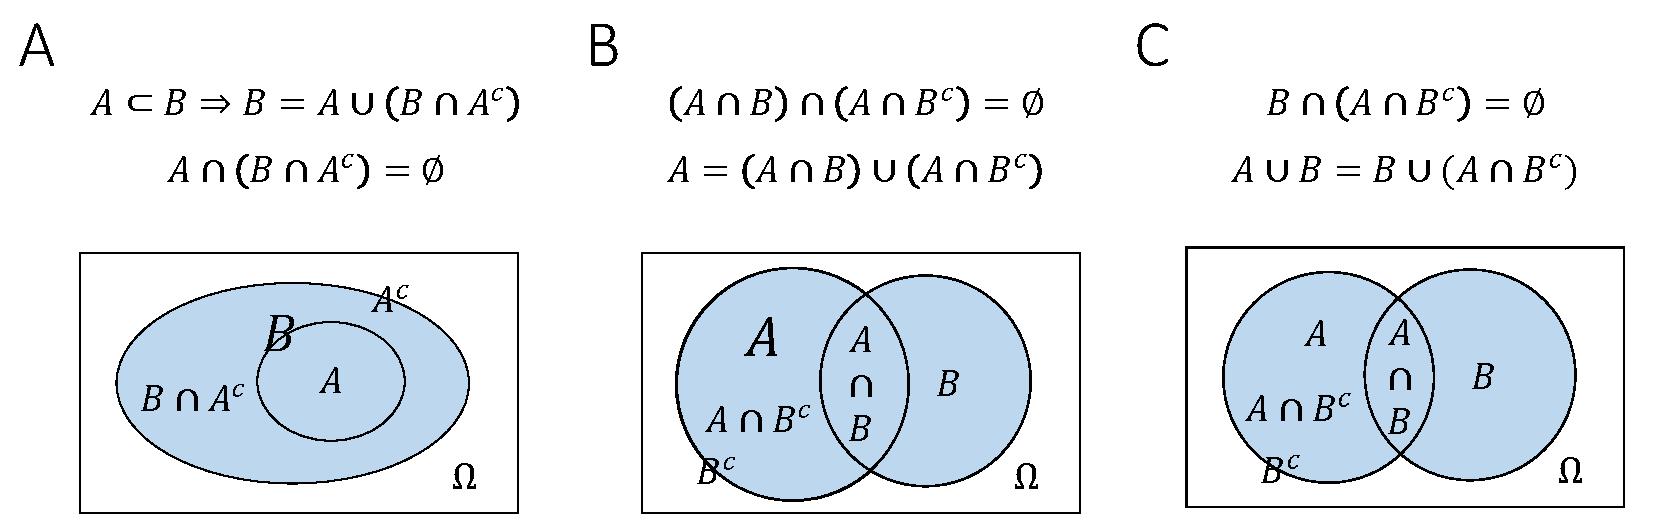
\includegraphics[width=0.9\linewidth]{3_Abbildungen/wtfi_3_venn_diagramme} \end{center}
\vspace{1mm}

Zu 1.: Wir halten zunächst fest, dass aus \(A^c := \Omega \setminus A\)
folgt, dass \(A^c \cup A = \Omega\) und dass \(A^c \cap A = \emptyset\).
Mit der Nomiertheit und der \(\sigma\)-Additivität von \(\mathbb{P}\)
folgt dann \begin{equation}
\mathbb{P}(\Omega) = 1
\Leftrightarrow
\mathbb{P}(A^c \cup A) = 1
\Leftrightarrow
\mathbb{P}(A^c) + \mathbb{P}(A)  = 1
\Leftrightarrow
\mathbb{P}(A^c) = 1 - \mathbb{P}(A).
\end{equation}
\end{frame}

\begin{frame}{Weitere Eigenschaften}
\protect\hypertarget{weitere-eigenschaften-2}{}
\footnotesize
\setstretch{1.1}

\underline{Beweis (fortgeführt)}

Zu 2.: Zunächst gilt (vgl. Abbildung A) \begin{equation}
A \subset B \Rightarrow B = A \cup (B \cap A^c)
\mbox{ mit } A \cap (B \cap A^c) = \emptyset.
\end{equation} Mit der \(\sigma\)-Additivät von \(\mathbb{P}\) folgt
dann aber \begin{equation}
\mathbb{P}(B) = \mathbb{P}(A) + \mathbb{P}(B \cap A^c).
\end{equation} Mit \(\mathbb{P}(B \cap A^c) \ge 0\) folgt dann
\(\mathbb{P}(A) \le \mathbb{P}(B)\).

Zu 3.: Zunächst gilt (vgl. Abbildung B) \begin{equation}
(A \cap B) \cap (A \cap B^c)  = \emptyset
\mbox{ und } A  = (A \cap B) \cup (A \cap B^c).
\end{equation} Mit der \(\sigma\)-Addivität von \(\mathbb{P}\) folgt
dann \begin{align}
\begin{split}
\mathbb{P}(A) = \mathbb{P}(A \cap B) + \mathbb{P}(A \cap B^c)
\Leftrightarrow
\mathbb{P}(A \cap B)
= \mathbb{P}(A) - \mathbb{P}(A \cap B^c)
\end{split}
\end{align}

Zu 4.: Zunächst gilt (vgl. Abbildung C) \begin{equation}
B \cap (A \cap B^c)  = \emptyset
\mbox{ und } A \cup B = B \cup (A \cap B^c).
\end{equation} Mit der \(\sigma\)-Addivität von \(\mathbb{P}\) folgt
dann \begin{equation}
\mathbb{P}(A \cup B) = \mathbb{P}(B) + \mathbb{P}(A \cap B^c).
\end{equation} Mit 3. folgt dann \begin{equation}
\mathbb{P}(A \cup B) = \mathbb{P}(B) + \mathbb{P}(A) - \mathbb{P}(A \cap B)
\end{equation}

Zu 5.: Die Aussage folgt direkt aus 4. mit
\(\mathbb{P}(A \cap B) = \emptyset\) und \(\mathbb{P}(\emptyset) = 0\).
\(\hfill\Box\)
\end{frame}

\begin{frame}{}
\protect\hypertarget{section-8}{}
\setstretch{2}
\vfill
\large

Interpretation

Gemeinsame Wahrscheinlichkeiten

Weitere Eigenschaften

\textbf{Unabhängige Ereignisse}

Bedingte Wahrscheinlichkeiten

Selbstkontrollfragen \vfill
\end{frame}

\begin{frame}{Unabhängige Ereignisse}
\protect\hypertarget{unabhuxe4ngige-ereignisse}{}
\setstretch{1.2}
\small
\begin{definition}[Unabhängige Ereignisse]
\justifying
Zwei Ereignisse $A \in \mathcal{A}$ and $B \in \mathcal{A}$ heißen
\textit{(stochastisch) unabhängig}, wenn
\begin{equation}
\mathbb{P}(A \cap B) = \mathbb{P}(A)\mathbb{P}(B).
\end{equation}
Eine Menge von Ereignissen $\{A_i|i \in I\}\subset \mathcal{A}$ mit beliebiger
Indexmenge $I$ heißt (stochastisch) unabhängig, wenn für jede endliche Untermenge
$J \subseteq I$ gilt, dass
\begin{equation}
\mathbb{P}\left(\cap_{j \in J} A_j \right) = \prod_{j \in J}\mathbb{P}(A_j).
\end{equation}
\end{definition}
\vspace{-2mm}
\footnotesize

Bemerkungen \vspace{-1mm}

\begin{itemize}
\justifying
\itemsep1mm
\item Die Unabhängigkeit bestimmter Ereignissen kann in der Definition eines
probabilistischen Modells vorausgesetzt werden, so zum Beispiel die Unabhängigkeit
von Fehlervariablen in statistischen Modellen.
\item Die Unabhängigkeit von Ereignissen kann aus der Definition eines probabilistischen Modells folgen.
\item Disjunkte Ereignisse mit von Null verschiedener Wahrscheinlichkeit sind nie unabhängig:
\item[] $\quad\quad\quad \mathbb{P}(A)\mathbb{P}(B) > 0$, aber $\mathbb{P}(A \cap B) = \mathbb{P}(\emptyset) = 0$, also
$\mathbb{P}(A \cap B) \neq \mathbb{P}(A)\mathbb{P}(B)$.
\item Die Bedingung der beliebigen Untermengen von $I$ sichert die paarweise unabhängig der $A_i, i \in I$.
\item Der Sinn der Produkteigenschaft bei Unabhängkeit erschließt sich im Kontext \textit{bedingter Wahrscheinlichkeiten}.
\end{itemize}
\end{frame}

\begin{frame}{}
\protect\hypertarget{section-9}{}
\setstretch{2}
\vfill
\large

Interpretation

Gemeinsame Wahrscheinlichkeiten

Weitere Eigenschaften

Unabhängige Ereignisse

\textbf{Bedingte Wahrscheinlichkeiten}

Selbstkontrollfragen \vfill
\end{frame}

\begin{frame}{Bedingte Wahrscheinlichkeiten}
\protect\hypertarget{bedingte-wahrscheinlichkeiten}{}
\small
\begin{definition}[Bedingte Wahrscheinlichkeit]
\justifying
$(\Omega,\mathcal{A}, \mathbb{P})$ sei ein Wahrscheinlichkeitsraum und $A, B\in \mathcal{A}$
seien Ereignisse mit $\mathbb{P}(B) > 0$. Die \textit{bedingte Wahrscheinlichkeit des Ereignisses
$A$ gegeben das Ereignis $B$} ist definiert als
\begin{equation}
\mathbb{P}(A|B) := \frac{\mathbb{P}(A \cap B)}{\mathbb{P}(B)}.
\end{equation}
Weiterhin heißt das für ein festes $B \in \mathcal{A}$ mit $\mathbb{P}(B) > 0$ 
definierte Wahrscheinlichkeitsmaß
\begin{equation}
\mathbb{P}(\,\,|B) : \mathcal{A} \to [0,1],
A \mapsto \mathbb{P}(A|B) := \frac{\mathbb{P}(A \cap B)}{\mathbb{P}(B)}
\end{equation}
die \textit{bedingte Wahrscheinlichkeit gegeben Ereignis $B$}.
\end{definition}
\end{frame}

\begin{frame}{Bedingte Wahrscheinlichkeiten}
\protect\hypertarget{bedingte-wahrscheinlichkeiten-1}{}
\small
\setstretch{1.5}

Bemerkungen

\begin{itemize}
\itemsep1mm
\item $\mathbb{P}(A|B)$ ist die mit $1/\mathbb{P}(B)$ skalierte gemeinsame Wahrscheinlichkeit $\mathbb{P}(A \cap B)$.
\item Die Festlegung der gemeinsamen Wahrscheinlichkeit $\mathbb{P}(A \cap B)$ legt $\mathbb{P}(A|B)$ schon fest.
\item Im Gegensatz zu $\mathbb{P}(\cdot \cap B)$ definiert $\mathbb{P}(\cdot \vert B)$ ein Wahrscheinlichkeitsmaß für alle $A \in \mathcal{A}$.
\item Es gelten also 
\begin{itemize}
\begin{small}
\item[$\circ$] $\mathbb{P}(A|B) \ge 0$ für alle $A \in \mathcal{A}$,
\item[$\circ$] $\mathbb{P}(\Omega|B) =  1$ und 
\item[$\circ$] $\mathbb{P}\left(\cup_{i=1}^\infty A_i|B \right) = \sum_{i=1}^\infty \mathbb{P}(A_i|B)$ für  paarweise disjunkte $A_1,A_2,... \in \mathcal{A}$.
\end{small}
\end{itemize}
\item $\Rightarrow$ Die Rechenregeln der Wahrscheinlichkeitstheorie gelten für die Ereignisse links des Strichs. 
\item Üblicherweise gilt $\mathbb{P}(A|B) \neq \mathbb{P}(B|A)$, z.B. 
\begin{equation*}
\mathbb{P}(\mbox{Tod}|\mbox{Erhängen}) \neq  \mathbb{P}(\mbox{Erhängen}|\mbox{Tod}).
\end{equation*}
\item Eine Verallgemeinerung für $\mathbb{P}(B) = 0$ ist möglich, aber technisch aufwändig.
\end{itemize}
\end{frame}

\begin{frame}{Bedingte Wahrscheinlichkeiten}
\protect\hypertarget{bedingte-wahrscheinlichkeiten-2}{}
Beispiel \footnotesize \setstretch{1.3}

Wir betrachten erneut das Modell \((\Omega, \mathcal{A}, \mathbb{P})\)
des fairen Würfels. Wir wollen die bedingte Wahrscheinlichkeit für das
Ereignis ``Es fällt eine gerade Augenzahl'' gegeben das Ereignis ``Es
fällt eine Zahl größer als Drei'' berechnen. Wir haben oben bereits
gesehen, dass das Ereignis ``Es fällt eine gerade Augenzahl'' der
Teilmenge \(A := \{2,4,6\}\) von \(\Omega\) entspricht, und dass das
Ereignis ``Es fällt eine Zahl größer als Drei'' der Teilmenge
\(B := \{4,5,6\}\) von \(\Omega\) entspricht. Weiterhin haben wir
gesehen, dass unter der Annahme, dass der modellierte Würfel fair ist,
gilt, dass \begin{align}
\mathbb{P}(\{2,4,6\})
& = \mathbb{P}(\{2\}) + \mathbb{P}(\{4\}) + \mathbb{P}(\{6\})
= 1/6 + 1/6 + 1/6 = 3/6   \\
\mathbb{P}(\{4,5,6\})
& = \mathbb{P}(\{4\}) + \mathbb{P}(\{5\}) + \mathbb{P}(\{6\})
= 1/6 + 1/6 + 1/6 = 3/6.
\end{align} Schließlich hatten wir auch gesehen, dass das Ereignis
\(A \cap B\), also das Ereignis ``Es fällt eine gerade Augenzahl, die
größer als Drei ist'', die Wahrscheinlichkeit \begin{equation}
\mathbb{P}(A \cap B) = \mathbb{P}(\{2,4,6\} \cap \{4,5,6\}) = \mathbb{P}(\{4,6\})
= \mathbb{P}(\{4\}) + \mathbb{P}(\{6\}) = 1/6 + 1/6 = 2/6
\end{equation} hat. Nach Definition der bedingten Wahrscheinlichkeit
ergibt sich dann direkt \begin{equation}
\mathbb{P}(A|B)
= \frac{\mathbb{P}(A \cap B)}{\mathbb{P}(B)}
= \frac{\mathbb{P}(\{4,6\})}{\mathbb{P}(\{4,5,6\})}
= \frac{2/6}{3/6}
= 2/6 \cdot 6/3
= 2/3.
\end{equation} Wenn man also weiß, dass eine Augenzahl größer als Drei
gefallen ist, ist die Wahrscheinlichkeit, dass es sich dabei um eine
gerade Augenzahl handelt 2/3. Wenn man ersteres nicht weiß, ist die
Wahrscheinlichkeit für das Fallen einer geraden Augenzahl (nur) 1/2.
Dies Beispiel verdeutlicht insbesondere, dass das Bedingen auf einem
Ereignis der Inkorporation von neuem Wissen in
wahrscheinlichkeitstheoretische Modellen entspricht.
\end{frame}

\begin{frame}{Bedingte Wahrscheinlichkeiten}
\protect\hypertarget{bedingte-wahrscheinlichkeiten-3}{}
\small
\begin{theorem}[Bedingte Wahrscheinlichkeit unter Unabhängigkeit]
\normalfont
\justifying
$(\Omega,\mathcal{A}, \mathbb{P})$ sei ein Wahrscheinlichkeitsraum und 
$A,B\in \mathcal{A}$ seien unabhängige Ereignisse mit $\mathbb{P}(B) \ge 0$. 
Dann gilt
\begin{equation}
\mathbb{P}(A|B)
= \frac{\mathbb{P}(A \cap B)}{\mathbb{P}(B)}
= \frac{\mathbb{P}(A)\mathbb{P}(B)}{\mathbb{P}(B)}
= \mathbb{P}(A).
\end{equation}
\end{theorem}

\footnotesize

Bemerkungen

\begin{itemize}
\justifying
\item Bei Unabhängigkeit von $A$ und $B$ ist es irrelevant, ob auch $B$ eintritt,  $\mathbb{P}(A)$ bleibt gleich.
\item Stochastische Unabhängigkeit wird also als $\mathbb{P}(A)\mathbb{P}(B)$ modelliert, damit $\mathbb{P}(A|B) = \mathbb{P}(A)$ gilt.
\end{itemize}

\small

\(\Rightarrow\) Die stochastische Unabhängigkeit zweier Ereignisse
bedeutet, dass das Wissen um das Eintreten eines der beiden Ereignisse
die Wahrscheinlichkeit für das Eintreten des anderen Ereignisses nicht
ändert. Andersherum bedeutet stochastische Abhängigkeit, dass das Wissen
um das Eintreten eines der beiden Ereignisse die Wahrscheinlichkeit für
das Eintreten des anderen Ereignisses verändert, also erhöht oder
verringert.
\end{frame}

\begin{frame}{Bedingte Wahrscheinlichkeiten}
\protect\hypertarget{bedingte-wahrscheinlichkeiten-4}{}
\small
\begin{theorem}[Gemeinsame und bedingte Wahrscheinlichkeiten]
\normalfont
Es seien $(\Omega,\mathcal{A}, \mathbb{P})$ ein W-Raum und $A,B\in \mathcal{A}$
mit $\mathbb{P}(\cdot|B) \ge 0$. Dann gilt
\begin{equation}
\mathbb{P}(A \cap B)
= \mathbb{P}(A|B)\mathbb{P}(B)
= \mathbb{P}(B|A)\mathbb{P}(A).
\end{equation}
\end{theorem}

\footnotesize

\underline{Beweis}

Mit der Definition der jeweiligen bedingten Wahrscheinlichkeit folgen
direkt \begin{equation}
\mathbb{P}(A|B) = \frac{\mathbb{P}(A \cap B)}{\mathbb{P}(B)}
\Leftrightarrow 
\mathbb{P}(A \cap B) =\mathbb{P}(A|B)\mathbb{P}(B)
\end{equation} und \begin{equation}
\mathbb{P}(B|A) = \frac{\mathbb{P}(B \cap A)}{\mathbb{P}(A)}
\Leftrightarrow 
\mathbb{P}(A \cap B) =\mathbb{P}(B|A)\mathbb{P}(A).
\end{equation}

Bemerkung

\begin{itemize}
\tightlist
\item
  Gemeinsame Wahrscheinlichkeiten können aus bedingten und totalen
  Wahrscheinlichkeiten berechnet werden.
\item
  Definition von \(\mathbb{P}(A)\) und \(\mathbb{P}(B|A)\) definiert
  \(\mathbb{P}(A \cap B)\) implizit mit.
\end{itemize}
\end{frame}

\begin{frame}{Elementare Wahrscheinlichkeiten}
\protect\hypertarget{elementare-wahrscheinlichkeiten}{}
\small
\begin{theorem}[Gesetz der totalen Wahrscheinlichkeit]
\normalfont
\justifying
$(\Omega,\mathcal{A},\mathbb{P})$ sei ein Wahrscheinlichkeitsraum und $A_1, ...,A_k$
sei eine Partition von $\Omega$. Dann gilt 
für jedes $B \in \mathcal{A}$, dass
\begin{equation}
\mathbb{P}(B) = \sum_{i=1}^k \mathbb{P}(B|A_i)\mathbb{P}(A_i).
\end{equation}
\end{theorem}
\vspace{-1mm}

\footnotesize

\underline{Beweis}

Für \(i = 1,...,k\) sei \(C_i := B \cap A_i\), so dass
\(\cup_{i=1}^k C_i = B\) und \(C_i \cap C_j = \emptyset\) für
\(1 \le i,j \le k,i \neq j\).

\begin{minipage}{.29\linewidth}
\begin{center}

\begin{center}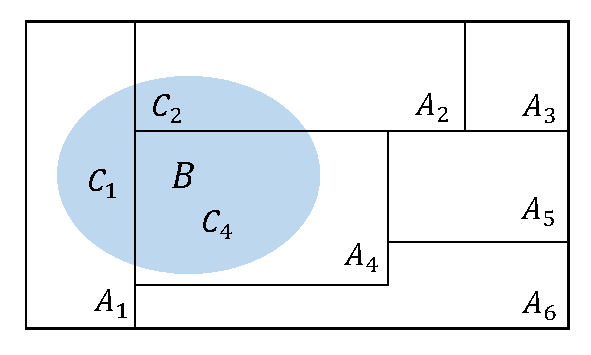
\includegraphics[width=0.7\linewidth]{3_Abbildungen/wtfi_3_partition} \end{center}
\end{center}
\end{minipage}
\begin{minipage}{.69\linewidth}
\begin{equation*}
\mbox{Also gilt }
\mathbb{P}(B)
= \sum_{i=1}^k \mathbb{P}(C_i)
= \sum_{i=1}^k \mathbb{P}(B \cap A_i)
= \sum_{i=1}^k \mathbb{P}(B|A_i)\mathbb{P}(A_i).
\end{equation*}
\end{minipage}

\(\hfill \Box\)

\vspace{-1mm}

Bemerkung

\begin{itemize}
\tightlist
\item
  Totale Wahrscheinlichkeiten können aus bedingten und totalen
  Wahrscheinlichkeiten berechnet werden.
\item
  \(\mathbb{P}(B)\) entspricht der gewichteten Summe der bedingten
  Wahrscheinlichkeiten \(\mathbb{P}(B|A_i)\) mit Gewichten
  \(\mathbb{P}(A_i)\).
\end{itemize}
\end{frame}

\begin{frame}{Elementare Wahrscheinlichkeiten}
\protect\hypertarget{elementare-wahrscheinlichkeiten-1}{}
\small
\begin{theorem}[Theorem von Bayes]
\normalfont
\justifying
$(\Omega,\mathcal{A},\mathbb{P})$ sei ein Wahrscheinlichkeitsraum und $A_1, ...,A_k$ 
sei eine Partition von $\Omega$ mit $\mathbb{P}(A_i) > 0$ für alle $i = 1,...,k$.
Wenn $\mathbb{P}(B) > 0$ gilt, dann gilt für jedes $i = 1,...,k$, dass
\begin{equation}
\mathbb{P}(A_i|B)
= \frac{\mathbb{P}(B|A_i)\mathbb{P}(A_i)}{\sum_{i=1}^k \mathbb{P}(B|A_i)\mathbb{P}(A_i)}.
\end{equation}
\end{theorem}

\footnotesize

\underline{Beweis} \vspace{1mm}

Mit der Definition der bedingten Wahrscheinlichkeit und dem Gesetz der
totalen Wahrscheinlichkeit gilt \begin{equation}
\mathbb{P}(A_i|B)
= \frac{\mathbb{P}(A_i \cap B)}{\mathbb{P}(B)}
= \frac{\mathbb{P}(B|A_i)\mathbb{P}(A_i)}{\mathbb{P}(B)}
= \frac{\mathbb{P}(B|A_i)\mathbb{P}(A_i)}{\sum_{i=1}^k \mathbb{P}(B|A_i)\mathbb{P}(A_i)}.
\end{equation} \(\hfill \Box\)
\end{frame}

\begin{frame}{Elementare Wahrscheinlichkeiten}
\protect\hypertarget{elementare-wahrscheinlichkeiten-2}{}
Bemerkungen \small

\begin{itemize}
\itemsep2mm
\item Das Theorem von Bayes ist eine zu $\mathbb{P}(A_i \cap B)/ \mathbb{P}(B)$ 
alternative Formel, um die bedingte Wahrscheinlichkeit  $\mathbb{P}(A_i|B)$ zu berechnen.
\item Das Theorem von Bayes gilt unabhängig von der Frequentistischen oder 
Bayesianischen Interpretation von Wahrscheinlichkeiten.
\item Im Rahmen der \textbf{Frequentistischen Inferenz} wird das Theorem von Bayes 
recht selten benutzt; hier steht vor allem die Tatsache $\mathbb{P}(A) = \mathbb{P}(A|B)$ 
bei Unabhängikeit von $A$ und $B$ im Vordergrund.
\item Im Rahmen der \textbf{Bayesianischen Inferenz} ist das Theorem von Bayes 
zentral; hier wird $\mathbb{P}(A_i)$ oft \textit{Prior Wahrscheinlichkeit} 
und $\mathbb{P}(A_i|B)$ oft \textit{Posterior Wahrscheinlichkeit des Ereignisses $A_i$} 
genannt. Wie oben erläutert entspricht $\mathbb{P}(A_i|B)$ dann der aktualisierten 
Wahrscheinlichkeit von $A_i$, wenn man um das Eintreten von $B$ weiß.
\end{itemize}
\end{frame}

\begin{frame}{}
\protect\hypertarget{section-10}{}
\setstretch{2}
\vfill
\large

Interpretation

Gemeinsame Wahrscheinlichkeiten

Weitere Eigenschaften

Unabhängige Ereignisse

Bedingte Wahrscheinlichkeiten

\textbf{Selbstkontrollfragen} \vfill
\end{frame}

\begin{frame}{Selbstkontrollfragen}
\protect\hypertarget{selbstkontrollfragen}{}
\setstretch{1.3}
\footnotesize
\begin{enumerate}
\item Erläutern Sie die Frequentistische Interpretation der Wahrscheinlichkeit eines Ereignisses.
\item Erläutern Sie die Bayesianische Interpretation der Wahrscheinlichkeit eines Ereignisses.
\item Geben Sie die Definition der gemeinsamen Wahrscheinlichkeit zweier Ereignisse wieder.
\item Erläutern Sie die intuitive Bedeutung der gemeinsamen Wahrscheinlichkeit zweier Ereignisse.
\item Geben Sie das Theorem zu weiteren Eigenschaften von Wahrscheinlichkeiten wieder.
\item Geben Sie die Definition der Unabhängigkeit zweier Ereignisse wieder.
\item Geben Sie die Definition der bedingten Wahrscheinlichkeit eines Ereignisses und der bedingten Wahrscheinlichkeit wieder.
\item Geben Sie das Theorem zur bedingten Wahrscheinlichkeit unter Unabhängigkeit wieder.
\item Erläutern Sie den Begriff der stochastischen Unabhängigkeit vor dem Hintergrund des Theorems zur bedingten Wahrscheinlichkeit unter Unabhängigkeit.
\item Geben Sie das Theorem zu gemeinsamen und bedingten Wahrscheinlichkeiten wieder.
\item Geben Sie das Gesetz von der totalen Wahrscheinlichkeit wieder.
\item Geben Sie das Theorem von Bayes wieder.
\item Erläutern Sie das Theorem von Bayes im Rahmen der Bayesianischen Inferenz.
\item Beweisen Sie das Theorem von Bayes.
\end{enumerate}
\end{frame}

\end{document}
